\chapter{Implementazione} \label{ch:implementazione} % 3

In questo capitolo viene discussa l'implementazione dei modelli presentati nel capitolo \ref{ch:modello}, evidenziando le diverse strategie adottate per affrontare alcune problematiche.
In particolar modo, verrà data rilevanza alle tecniche e alle strutture dati impiegate nel calcolo dell'esplorazione, riportando le varianti utilizzate durante il processo di sperimentazione del modello, quali i vari metodi di valutazione del guadagno di esplorazione di un punto campionato da un agente (Sezione \ref{sec:valutazione_esplorazione}).

Il codice del sistema e delle simulazioni, così come la cronologia delle modifiche, è disponibile su GitHub nel seguente repository: 

\href{https://github.com/leonardo-guglielmi/Multiagent-exploration-system.git}{\textsf{https://github.com/leonardo-guglielmi/Multiagent-exploration-system.git}}

Il linguaggio di programmazione utilizzato è 
%\href{https://www.python.org/about/}{\textbf{Python}}, 
\textbf{Python}, 
che grazie alla sua semplicità e alla vasta gamma di librerie disponibili si rende particolarmente adatto alle fasi prototipali di un progetto.

\section{Schema del progetto} \label{sec:schema_classi}

In Figura \ref{fig:uml_scheme} si riporta il diagramma UML delle classi del progetto (per la sua realizzazione è stato utilizzato il tool online 
%\href{https://app.diagrams.net/}{\textbf{draw.io}}
\textbf{draw.io}).

\begin{figure}[p]
    \centering
    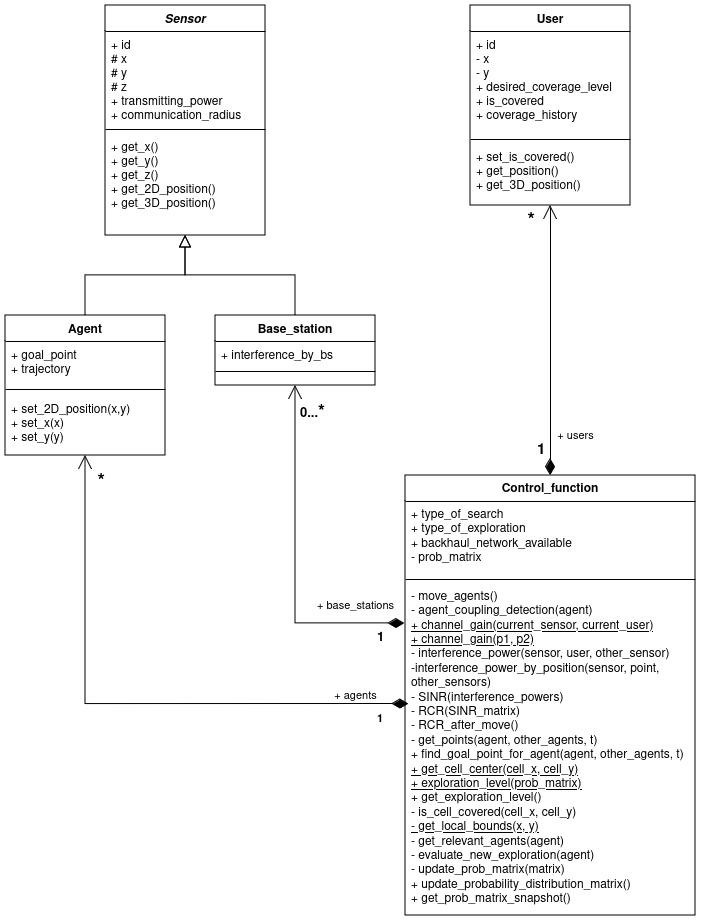
\includegraphics[width=1\textwidth]{img/ch3/UML_thesis.png}
    \caption[Schema UML]{Schema UML della classi usate nella simulazione}
    \label{fig:uml_scheme}
\end{figure}

\subsection{Classi \texttt{Sensor, Agent e Base\_stations}} \label{subsec:sensors}
La classe \texttt{Sensor} rappresenta un sensore, astraendo le differenze tra agente e BS.
Contiene le caratteristiche comuni ai due elementi del sistema, ovvero la posizione tridimensionale \texttt{(x,y,z)}; la potenza di trasmissione \texttt{trasmitting\_power}; il raggio di esplorazione \texttt{exploration\_radius}, implementati come attributi della classe.
La classe \texttt{Agent} estende \texttt{Sensor}, aggiungendovi gli attributi propri degli agenti, ovvero \texttt{trajectory}, una lista cronologica delle posizioni occupate dall'agente, e \texttt{goal\_point}, il punto obiettivo che l'agente vuole raggiungere in un certo istante di tempo.
La classe \texttt{Base\_station} estende anch'essa \texttt{Sensor}, ed aggiunge semplicemente un attributo booleano \texttt{interference\_by\_bs}: se impostato a \texttt{True}, indica che il segnale di quella BS interferisce con quello degli \texttt{Agent}. Questo flag è stato aggiunto poiché, in molti casi reali, le frequenze sui cui operano i due sensori sono diverse e non interferiscono tra di loro. % 3.1.1
\subsection{Classe \texttt{User}} \label{subsec:user}

La classe \texttt{User} rappresenta un utente a terra a cui deve essere fornita copertura.
Gli attributi rilevanti sono la posizione \texttt{(x,y)}; il livello di SINR \texttt{desired\_coverage\_level} tale che l'utente sia considerato coperto; il booleano \texttt{is\_covered}, che indica se in un certo istante di tempo tale utente è coperto o meno; una lista \texttt{coverage\_history} che contiene la cronologia dello stato di copertura dell'utente nel tempo. % 3.1.2
\subsection{Classe \texttt{Control\_function}} \label{subsec:control_function}
Questa classe contiene i metodi utilizzati dalla funzione di controllo.
Al suo interno sono presenti i riferimenti a tutti gli attori del sistema: troviamo infatti una lista di \texttt{Agent}, una di \texttt{Base\_station} e una di \texttt{User}.
Inoltre, contiene tutta una serie di attributi usati durante i processi decisionali, come il criterio per la scelta tra i punti campionati, oppure la matrice di probabilità utilizzata per l'esplorazione, descritta meglio in  \ref{subsec:mappa_prob}.

\subsubsection{Metodo  \texttt{move\_agents()}}
Questa funzione, mostrata nello Snippet \ref{snip:move_agents}, esegue lo spostamento degli agenti come descritto in \ref{sec:algoritmo_controllo}.
Inoltre, nel caso in cui venga riconosciuta una situazione di accoppiamento tra agenti, viene applicata una deviazione; tale processo è descritto approfonditamente in \ref{sec:controllo_accoppiamento_agenti}.

\lstinputlisting[
    language=Python 
    , label= {snip:move_agents}
    , caption = {Funzione per lo spostamento degli agenti.}
    , frame=tb
    , belowcaptionskip=3mm
    , float = h
    ]
{code/move_agent_snip.py}

\subsubsection{Metodo \texttt{get\_points()}}
Dato un agente, questa funzione campiona un insieme di punti e ne restituisce un sottoinsieme secondo una certa regola.
Più precisamente, vengono campionati \texttt{NUM\_OF\_SAMPLES} punti secondo una \textbf{distribuzione normale}, centrata nell'attuale posizione dell'agente specificato.
Le strategie di selezione dei punti adottate sono le seguenti:
\begin{enumerate}

\item
Ricerca \textbf{systematic}: vengono considerati tutti i punti campionati. 
Questa strategia ha il problema che, occasionalmente, restituisce dei punti lontani dall'agente, e se tra questi vi fosse il punto ottimo, porterebbe l'agente a muoversi verso zone che, probabilmente, verrebbero esplorate prima da altri agenti, rendendo lo spostamento vano.

\item
Ricerca \textbf{local}: tra i punti campionati, vengono selezionati solo quelli che sono più vicini all'agente specificato rispetto ad altri sensori (Snippet \ref{snip:local_search}). Questa strategia predilige quindi un controllo locale dell'area, impedendo che un sensore vada a esplorare una zona che è più facilmente esplorabile da un altro.

\lstinputlisting[
    language=Python 
    , label= {snip:local_search}
    , caption = {Tecnica di selezione \textit{local}.}
    , frame=tb
    , belowcaptionskip=3mm
    , float = t
    ]
{code/local_search_snip.py}

\item
Ricerca \textbf{penalty}: come nella strategia \textit{local}, questa tecnica favorisce quei punti prossimi all'agente. A differenza della precedente non va ad escludere quelli più vicini ad altri, bensì va ad applicare una penalità ai livelli di $C(t)$ e $\Pi(t)$ calcolati in tali punti.

\pagebreak
\item
Ricerca \textbf{annealing forward}: riprendendo l'idea dell'algoritmo di ricerca locale \textit{simulated annealing}, si va ad aggiungere alla strategia \textit{local} una probabilità aggiuntiva, decrescente con il tempo, che il punto venga selezionato anche se è più vicino ad altri agenti. %(Snippet \ref{snip:annealing_search}).
Questa tecnica cerca di evitare lo stallo in punti di massimo locale.

\item
Ricerca \textbf{annealing reverse}: simile alla ricerca \textit{annealing forward}, in questa tecnica si va ad avere una probabilità crescente nel tempo. %(Snippet \ref{snip:annealing_search}).
In questo modo, con il passare del tempo, il valore atteso della lunghezza degli spostamenti aumenterà.
\end{enumerate}

%\lstinputlisting[
%    language=Python 
%    , label= {snip:annealing_search}
%    , caption = {Tecnica di selezione \textit{annealing forward} e \textit{annealing reverse}}
%    , frame=tb
%    , belowcaptionskip=3mm
%    , float = t
%    ]
%{code/annealing_search_snip.py}

\subsubsection{\texttt{find\_goal\_point\_for\_agent()}}
Dato un agente, questo metodo esamina tutti i punti forniti da \texttt{get\_points()}, più la posizione attuale dell'agente, cercando tra di essi l'ottimo.
Per fare ciò la posizione del sensore viene temporaneamente modificata con quella del punto in esame e viene ricalcolata la funzione obiettivo nella nuova configurazione del sistema; nel caso in cui il valore ottenuto sia il migliore trovato tale punto viene salvato come nuovo $p_i^*$.
Poiché la funzione obiettivo, come esposto nel capitolo \ref{ch:modello}, si divide in due parti, per valutare $R(t)$ nel nuovo punto dovranno essere calcolati nuovamente l'RCR e il valore di esplorazione.

\subsubsection{\texttt{is\_cell\_covered()}}
Questo metodo, fornite le coordinate di una cella di esplorazione, ritorna lo stato di copertura di quest'ultima.
Come indicato in \ref{sec:modello_esplorazione}, per determinare lo stato si prende come punto di riferimento il centro della cella; questo implica un'approssimazione sulla reale probabilità che in quella zona vi sia un utente, approssimazione che cresce all'aumentare della dimensione delle celle.

\input{files/ch3/classi progetto/mappa_probabilità}
\subsubsection{Funzione per l'esplorazione} \label{subsubsec:expl_funct}
Questa funzione (Snippet \ref{snip:expl_funct}), data la matrice di probabilità, va a calcolare il livello globale di esplorazione, andando a fare la media delle probabilità di tutte le celle e trasformando il risultato in modo che, ad una probabilità complessiva minore, venga associato un livello di esplorazione maggiore, rendendolo compatibile con un problema di massimizzazione (Formula \ref{eq:global_funct}).
\lstinputlisting[
language=Python 
, label={snip:expl_funct}
, caption={Funzione per il calcolo dell'esplorazione globale.}
, float = t
, frame=tb
, belowcaptionskip=3mm
]{code/global_expl_function.py}

Questo metodo può essere usato anche per valutare l'esplorazione in un punto campionato da un agente; tuttavia nella pratica quest'ultimo esplorerà solo quelle celle vicino al \texttt{goal\_point}, rendendo quindi il calcolo globale dell'esplorazione poco conveniente a causa del suo costo computazionale.
Per tale scopo sono stati quindi creati dei metodi di valutazione dell'esplorazione locale, descritti approfonditamente in \ref{sec:valutazione_esplorazione}. % 3.1.3 % 3.1
\section{Esecuzione concorrente} \label{subsec:concur_agents}

In un contesto reale, ciascun agente eseguirebbe la funzione obiettivo sul proprio sistema di calcolo in modo indipendente dagli altri.
Si è dunque ritenuto opportuno implementare un meccanismo di parallelizzazione per il calcolo del \texttt{goal\_point} di ciascun agente, riducendo sensibilmente i tempi di esecuzione delle simulazioni.
Data la presenza nell'interprete Python del \textit{Global Interpreter Lock}, la scelta del modulo da impiegare è ricaduta su \texttt{multiprocessing}, un package Python che espone delle API per la creazione e gestione di processi paralleli.

 Per parallelizzare la simulazione, si crea un processo distinto per ciascun agente, il quale eseguirà il metodo \texttt{goal\_point\_agent()}.
 Una volta calcolato il punto ottimo, il processo lo inserisce in un dizionario condiviso, associandogli come chiave l'id del proprio agente.
Una volta terminati tutti i processi agente, nel processo principale viene estratto dal dizionario ciascun \texttt{goal\_point} e associato al relativo agente (Snippet \ref{snip:concurrent_simu}).
\lstinputlisting[
language=Python 
, label = {snip:concurrent_simu}
, caption = {Esecuzione parallela della ricerca del \texttt{goal\_point}.}
, float = t
, frame = tb
, belowcaptionskip = 3mm
]{code/concurrent_simu.py} % 3.2
\section{Valutazione dell'esplorazione} \label{sec:valutazione_esplorazione}
Come accennato in \ref{subsubsec:expl_funct}, andare a valutare per ogni punto campionato l'esplorazione \textbf{globale} risulta estremamente costoso, implicando dei tempi di simulazione estremamente lunghi.
Inoltre, l'uso di questo approccio è poco utile; infatti dopo il movimento degli agenti nelle zone lontane dal punto campionato in esame avrò verosimilmente uno stato di esplorazione diverso, rendendo la previsione fatta su quelle celle durante la valutazione del punto ottimo poco attendibile.
A fronte di queste problematiche, durante le fasi sperimentali sono stati progettati e implementati diversi metodi per valutare localmente il livello di esplorazione di un punto, in modo che tale operazione risulti computazionalmente valida.

% metto prima il metodo finale, e poi le caratteristiche di quellli vecchi le ricollego a queste?
\subsection{Metodi sperimentali per la valutazione dell'esplorazione} \label{subsec:experimental_expl_eval}
In questa sotto-sezione si riportano i vari metodi sviluppati durante le fasi di test, ma che sono stati rimpiazzati da una versione successiva più accurata, fino ad arrivare a quello utilizzato negli esperimenti, ed esposto in \ref{subsec:expl_eval_frontier_NCC}.

\subsubsection{Simple Exploration}
Questo metodo è stato utilizzato nelle fasi iniziali per verificare la variazione di probabilità delle celle in tempi di simulazione ragionevoli. 
Esso non tiene conto del SINR per valutare la copertura di un cella, ma controlla soltanto che il suo centro sia abbastanza vicino ad un sensore.
Per ovvi motivi, tale metodo è stato rapidamente sostituito dai successivi.

\subsubsection{Local Square Interference Exploration (LSIE)}
In questa variante, si va a valutare la copertura di una cella tramite il livello di SINR calcolato nel suo centro, rendendo il requisito di copertura della cella simile a quello della copertura utente.
La novità principale è quella di non considerare tutte le celle della matrice, ma soltanto quelle che rientrano all'interno di un'area quadrata centrata nella posizione dell'agente, di lato \texttt{2$\cdot$EXPLORATION\_RADIUS} (Figura \ref{fig:esempio_LSIE}).
\begin{SCfigure}[1][h]
    \centering
    \caption[Esempio dell'area valutata con il metodo LSIE]{Esempio dell'area considerata dal metodo LSIE; si osserva come le celle presenti negli angoli dell'area siano difficilmente raggiungibili dal segnale dell'agente.}
    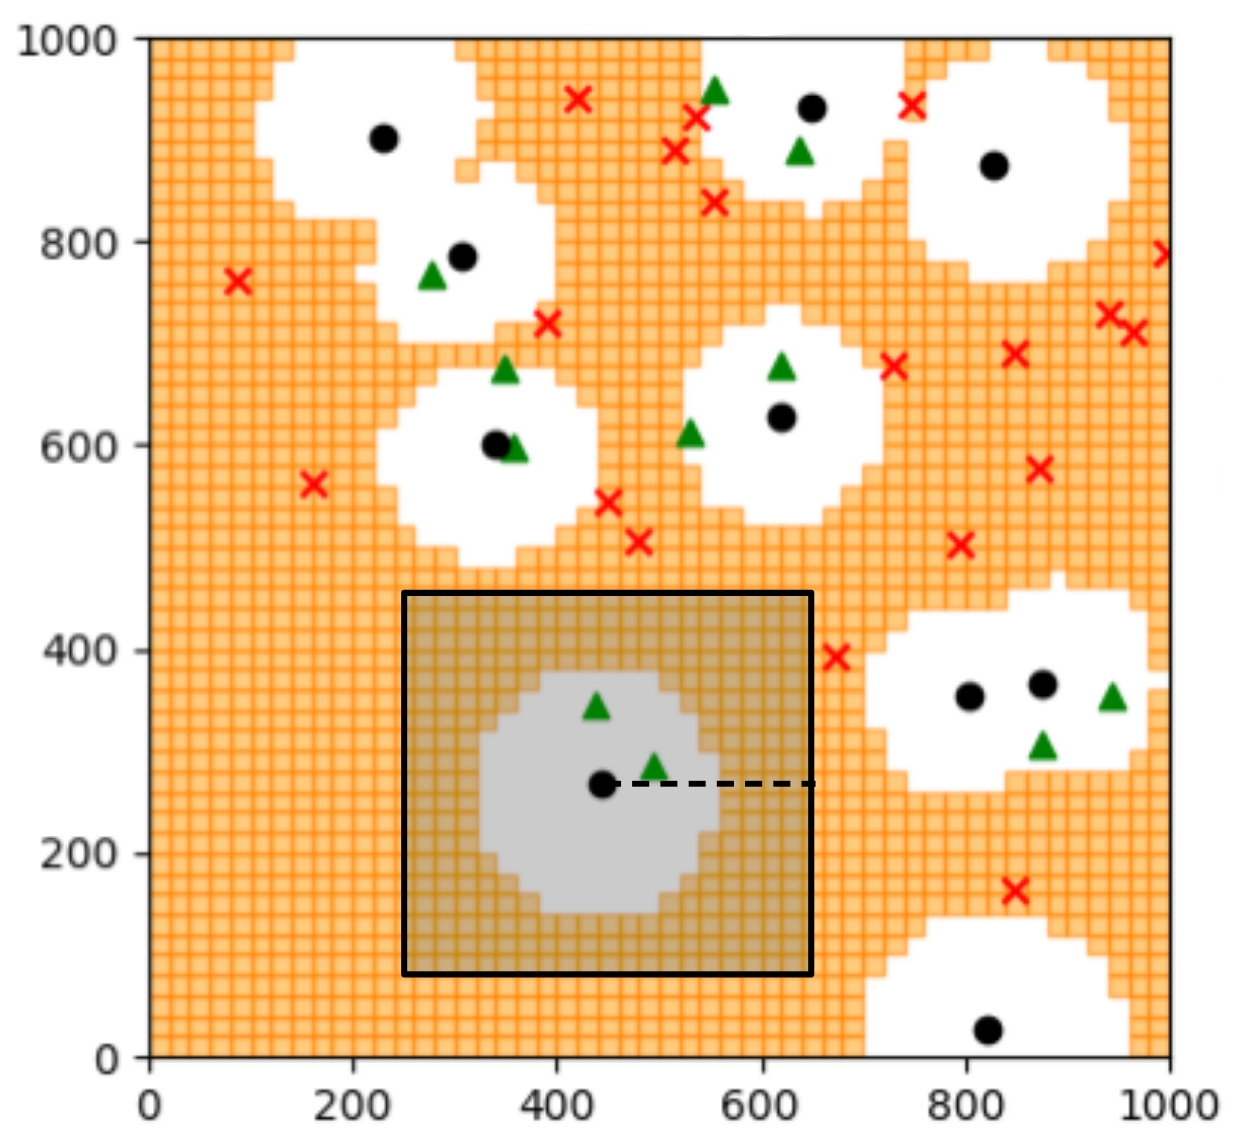
\includegraphics[width=0.5\textwidth]{img/ch3/esempio_LSIE.jpg}
    \label{fig:esempio_LSIE}
\end{SCfigure}

Inoltre si vanno a considerare soltanto le interferenze provenienti da sensori relativamente vicini all'agente, in quanto una eccessiva distanza rende il segnale d'interferenza trascurabile; questa considerazione permette di avere un minor numero di agenti nel calcolo del SINR, alleggerendo il costo computazionale.
Si osserva come la scelta del valore di \texttt{EXPLORATION\_RADIUS} sia critica, in quanto  un raggio maggiore implica una visione più approfondita dell'ambiente da parte dell'agente, comportando però una minore velocità del metodo.
\textbf{Sperimentalmente} si è osservato che ponendo \texttt{EXPLORATION\_RADIUS=200} si ha un'esplorazione completa dell'area intorno ad un punto, mantenendo un buon tempo di simulazione.
Il problema di questa variante è che, data la forma quadrata dell'area, si andranno a considerare anche le celle negli angoli, che molto probabilmente non saranno mai coperte dal segnale dell'agente (Figura \ref{fig:esempio_LSIE}).


\subsubsection{Local Circle Interference Exploration (LCIE)}
Rispetto al metodo precedente questa variante modifica la forma dell'area osservata, passando dall'utilizzo di un'area quadrata ad una circolare, rimuovendo quindi le celle che prima si trovavano negli angoli; questo porta ad un'ulteriore aumento di velocità del processo di valutazione, essendosi ridotto il numero di celle da osservare.
\begin{figure}[h]
    \centering
    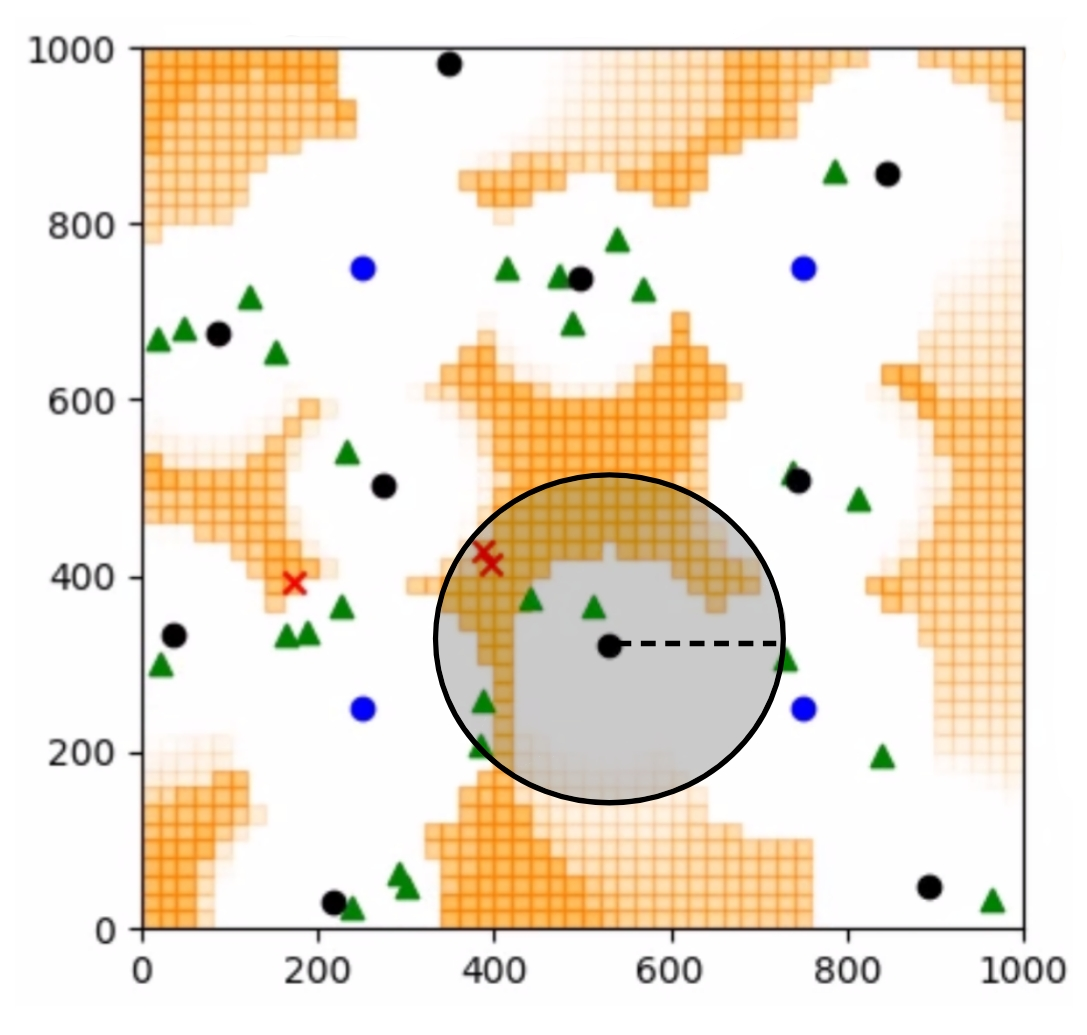
\includegraphics[width=0.5\textwidth]{img/ch3/esempio_LCIE.jpg}
    \caption[Esempio dell'area valutata con il metodo LCIE]{Esempio di area considerata dal metodo LCIE.}
    \label{fig:esempio_LCIE}
\end{figure}

\subsubsection{Local Square Interference Exploration, Neighbour Cell Control (LSIENCC)}
Implementata prima della \textit{Local Circle Interference Exploration}, questo metodo aggiunge una predizione sul livello di copertura di alcune celle quando sono soddisfatte alcune condizioni.
Tale predizione si basa sull'osservazione che, se il SINR calcolato in una cella è abbastanza alto, allora con molta probabilità anche quello delle celle adiacenti supererà la soglia richiesta.
Seguendo tale euristica, è possibile ridurre drasticamente i tempi di valutazione dell'esplorazione di quegli agenti isolati rispetto al resto della rete: infatti, la distanza da gli altri agenti fa sì che il livello di SINR rimanga abbastanza uniforme lungo l'area.
\subsection{Valutazione dell'esplorazione tramite frontiera con controllo delle celle adiacenti} \label{subsec:expl_eval_frontier_NCC}
Il metodo riportato in questa sotto-sezione è quello che verrà usato nelle simulazioni esposte nel Capitolo \ref{ch4:simulazioni}.
Esso è la combinazione delle varianti \textit{LCIE} e \textit{LSIENCC}, esposte nella sotto-sezione precedente; tale metodo include dunque i vantaggi di avere una regione da valutare il più ridotta possibile, senza però rinunciare alla precisione della stima, e di poter predire il livello di copertura di alcune celle, senza doverne calcolare esplicitamente il valore.

% da ricontrollare
I passaggi principali in cui l'algoritmo si articola sono i seguenti:
\begin{enumerate}[wide]


\item
Per prima cosa, il metodo seleziona quelle celle che rientrano nell'area da valutare, inserendo le informazioni rilevanti (posizione del centro e probabilità) in una struttura dati simile ad una matrice, ma con lunghezza delle righe variabile (Snippet \ref{snip:init_expl_eval}).
Inoltre, identifica gli agenti abbastanza vicini al punto campionato.
\lstinputlisting[
language=Python 
, label={snip:init_expl_eval}
, caption={Inizializzazione del metodo LCIENCC.}
, frame=tb
, float = ht
, belowcaptionskip=3mm
]{code/init_expl_eval_method.py}


\item
Successivamente, per ogni cella inclusa, calcola il SINR di ciascun agente precedentemente selezionato.
Dal calcolo del SINR vengono escluse quelle celle aventi $P_k=0$,  in quanto sono già coperte, e non apporterebbero nessun contributo all'esplorazione (Snippet \ref{snip:core_expl_eval}).
Se il livello di SINR di una cella supera una certa soglia \texttt{NEIGHBOUR\_SINR\_THRESHOLD}, la cella sovrastante e quella a destra (quella sotto e quella a sinistra sono state già esaminate) vengono inserite in \texttt{already\_checked\_cells}, ossia una lista che permette di escludere tali celle dalla valutazione del livello di SINR.
Prima di tale inserimento, viene fatta una serie di controlli per escludere quelle celle che eccedono l'aera di valutazione, e per evitare di etichettare come coperta una cella avente probabilità zero. 
\lstinputlisting[
language=Python 
, label={snip:core_expl_eval}
, caption={Calcolo della copertura nel metodo LCIENCC.}
, frame=tb
, float = p
, belowcaptionskip=3mm
]{code/core_expl_eval_method.py}


\item
Infine si calcola il livello di esplorazione, basandosi sulla matrice che associa a ciascuna cella il valore di SINR di ogni agente. (Snippet \ref{snip:final_expl_eval}).
\lstinputlisting[
language=Python 
, label={snip:final_expl_eval}
, caption={Valutazione dell'esplorazione nel metodo LCIENCC.}
, frame=tb
, float = h
, belowcaptionskip=3mm
]{code/final_expl_eval_method.py}


\end{enumerate} % 3.3
%\pagebreak
\section{Peso dell'esplorazione variabile} \label{sec:peso_esplorazione}
Il termine $\rho$, presente nell'Equazione \ref{eq:objective_function}, è un coefficiente che  indica l'importanza del processo di esplorazione all'interno dell'obiettivo globale.
Poiché la copertura degli utenti è l'obiettivo primario, inizialmente si è deciso di dare all'esplorazione una rilevanza minore, in modo che vengano favorite quelle azioni maggiormente orientate alla copertura; è stato dunque impostato un \textbf{peso constante} \texttt{EXPLORATION\_WEIGHT} (Snippet \ref{snip:expl_weight}), strettamente minore di 1.

\lstinputlisting[
language=Python 
, label={snip:expl_weight}
, caption = {varianti di peso dell'obiettivo di esplorazione}
, float = h
, frame=tb
, belowcaptionskip=3mm
]{code/expl_weight.py}

Successivamente è stato osservato come, nelle fasi iniziali, solitamente il valore di RCR fosse basso, risultando quindi sfavorevole incentivare la copertura di pochi utenti, rispetto alla ricerca di nuovi.
Per evitare tale comportamento, è stato implementato un \textbf{coefficiente di esplorazione decrescente} al crescere del numero di utenti coperti (Snippet \ref{snip:expl_weight}), ma indipendente dal loro totale, che permette di dare una rilevanza maggiore all'obiettivo di esplorazione nelle fasi iniziali, e ridurne il peso all'aumentare degli utenti coperti, applicando nuovamente un approccio più conservativo.
Inizialmente, come si vede in Figura \ref{fig:expl_weight_comparison}, quando la configurazione dei sensori ha un livello di RCR basso, l'importanza della funzione di esplorazione sarà relativamente elevata, per poi decrescere rapidamente; così facendo si ottiene un approccio flessibile alla configurazione attuale del sistema.

\begin{figure}
    \centering
    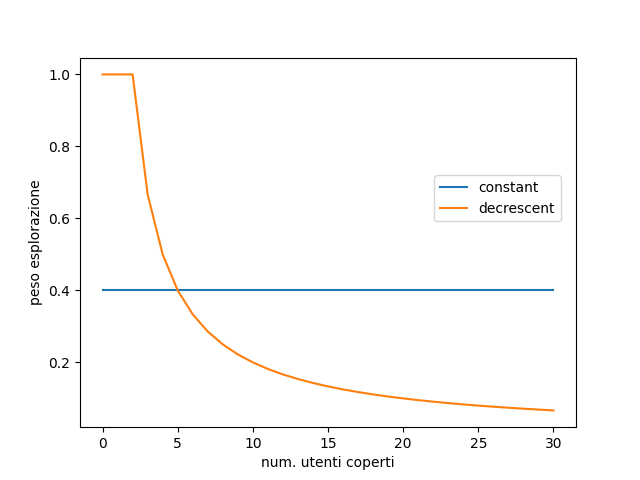
\includegraphics[width=0.8\textwidth]{img/ch3/expl_weight_comparison.png}
    \caption{Confronto tra i due tipi di peso al variare del numero di utenti coperti}
    \label{fig:expl_weight_comparison}
\end{figure}
\pagebreak
\section{Controllo per il disaccoppiamento di agenti} \label{sec:controllo_accoppiamento_agenti}

L'accoppiamento è un fenomeno causato dalla ridotta distanza tra due o più agenti, e provoca una minore capacità di copertura ed esplorazione da parte dei soggetti coinvolti.
Tale problematica si verifica quando agenti molto vicini identificano ripetutamente la stessa direzione di spostamento, causando un allineamento delle loro traiettorie; questo fa sì che il loro raggio di copertura si riduca a causa delle interferenze mutue.
Ciò ha come effetto quello di restringere l'orizzonte osservabile dagli agenti e conseguentemente un aumento della probabilità che gli agenti selezionino lo stesso punto ottimo.

\begin{figure}[t]
    \centering
    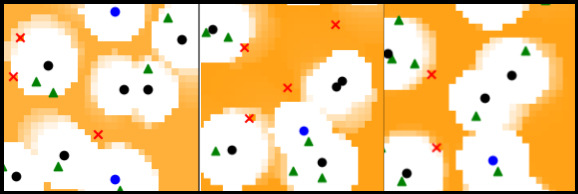
\includegraphics[width=0.8\textwidth]{img/ch3/agent_coupling_event.png}
    \caption[Esempio di accoppiamento tra agenti]{Un esempio di agenti accoppiati, rispettivamente negli istanti 15, 50 e 95. Si vede come, anche se la problematica sembra risolversi alla fine, essa ha drasticamente limitato il contributo degli agenti coinvolti.}
    \label{fig:agent_coupling_event}
\end{figure}

Per cercare di limitare la durata dell'accoppiamento è stato implementata una funzione in grado di riconoscere l'evento ed intervenire, cercando di orientare gli agenti coinvolti in direzioni opposte (Snippet \ref{snip:coupling_detection}).
\pagebreak
L'algoritmo implementato riconosce l'accoppiamento controllando ad ogni iterazione le posizioni pregresse degli agenti, confrontando le distanze mutue con un valore di soglia; nel caso questo venga raggiunto si crea una deviazione che cerca di allontanare gli agenti coinvolti.

\begin{SCfigure}[0.7][h]
    \centering
    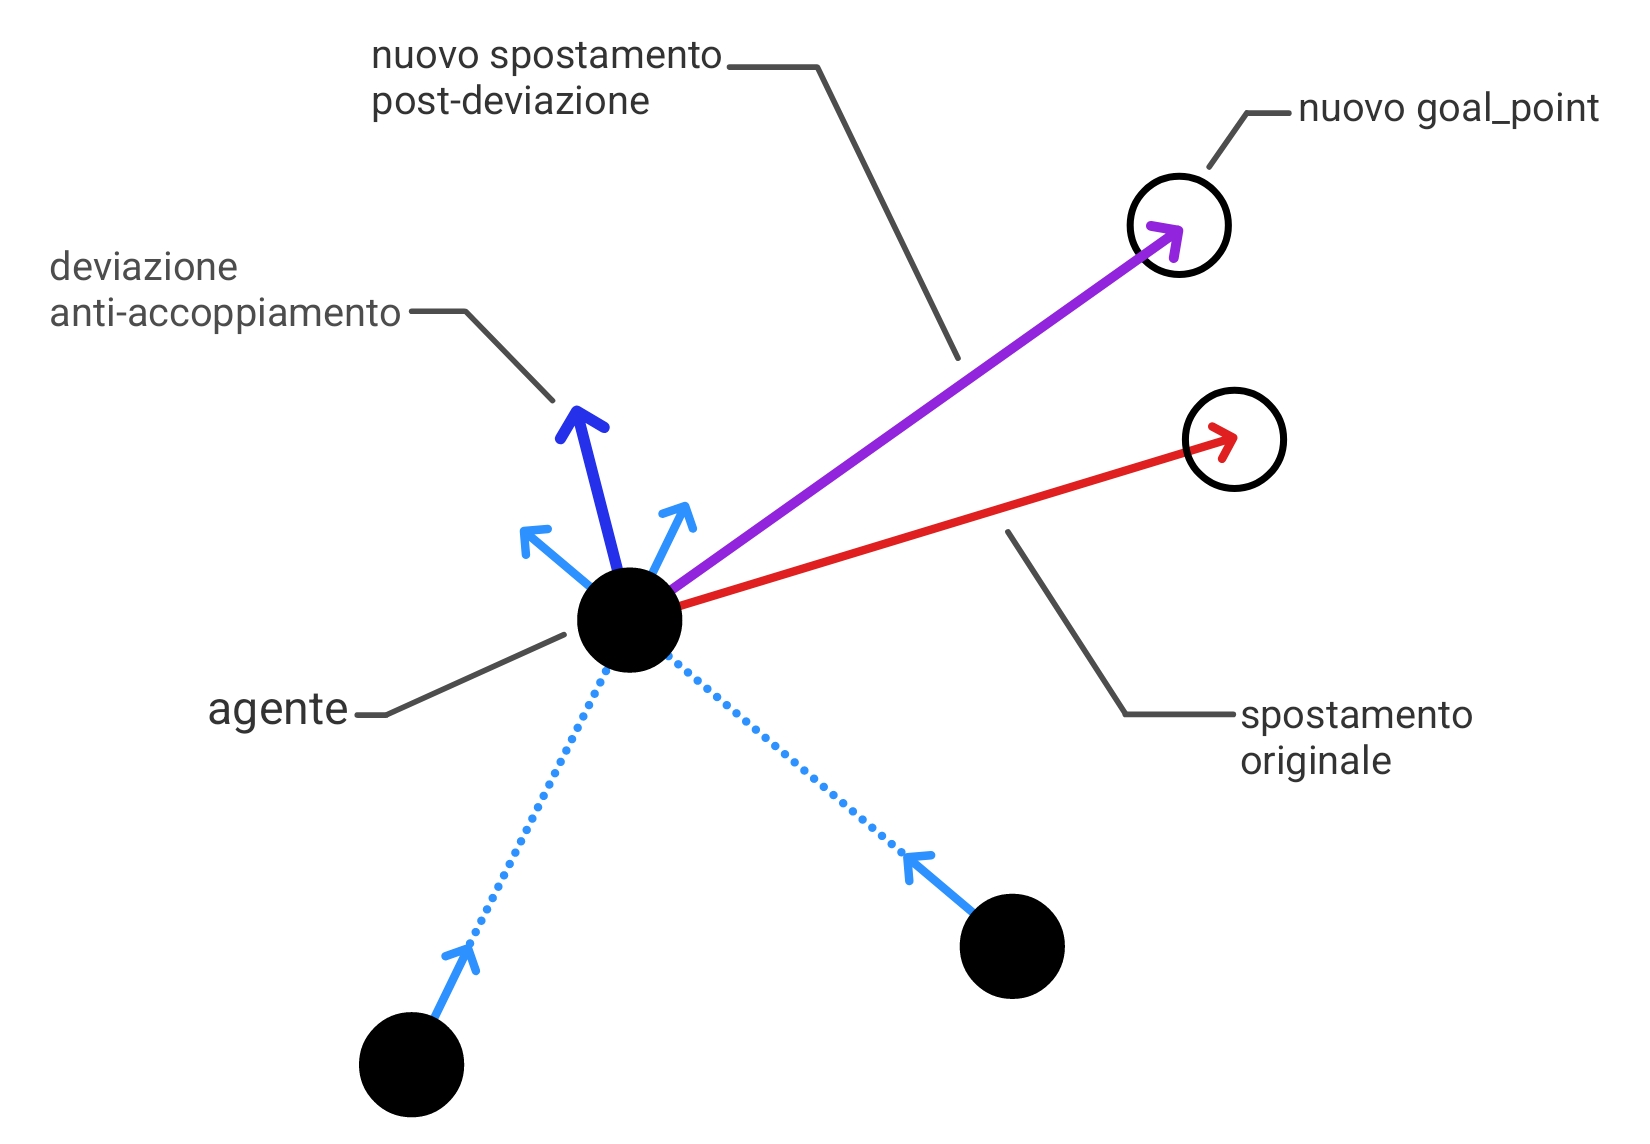
\includegraphics[width=0.6\textwidth]{img/ch3/schematic_anticoupling_system.jpg}
    \caption{Rappresentazione schematica del sistema anti-accoppiamento}
    \label{fig:schematic_decoupling_system}
\end{SCfigure}


Tale deviazione viene applicata sommandola alla direzione di spostamento del punto ottimo, come se fosse presente una forza repulsiva che agisce quando degli agenti sono vicini da troppo tempo (Figura \ref{fig:schematic_decoupling_system}).

\lstinputlisting[
    language=Python 
    , label= {snip:coupling_detection}
    , caption = {Funzione per il riconoscimento dell'accoppiamento.}
    , frame=tb
    , belowcaptionskip=3mm
    , float = p
    ]
{code/coupling_detection_system.py} % 3.4
